\chapter{User documentation}
\label{chap:udoc}
In the last chapter of the thesis, we first describe how to install the program and then show how to make the program generate random matrices or to test whether a certain matrix avoids a given forbidden pattern.

\section{Installation}
The program is written in C++, using the C++11 standard and is independent of any platform or compiler extensions. To use it, you either just use an executable file (Windows) or build the program using a C++ compiler.

\subsection{Windows}
Windows users can run the application using an executable file ``matrix-win.exe'' either directly, in which case the default configuration file will be used, or using command line with an optional parameter specifying the configuration file.

For those who want to alter the code (\cite{program}) or recompile the program in Visual Studio, Project File is also added.

\subsection{Unix, Linux, MacOS}
Users on other platforms than Windows can build the solution using command line easily by running ``./build.sh'', which uses the g++ compiler. Compiler can be switched by rewriting ``g++'' to some other variant (for example clang) in build.sh file. This leads to creating a an executable file ``matrix.exe'' which can be run with an optional parameter specifying the configuration file.

\section{Configuration file}
In order to modify what the program computes, we use a configuration file. The configuration file can be chosen when running the program in command line and relative path to it is the first (and only) option. If no path is inserted, the configuration file is expected to be located in the same directory as the executable file and its name is ``config.txt''.

The file is a standard text file, which can be modified by any text editor, and is structured into four sections:
\begin{itemize}
\item input
\item pattern
\item output
\item statistics
\end{itemize}
The order of the sections is not fixed and there can be additional empty lines for better readability. In each section, there is a list of options that can be set. There is at most one command of format ``option=value'' per line and there might be additional white spaces surrounding the ``='' sign.

If an option is set more than once, the latter value is always used. If, on the other hand, an option is not set at all, the default value is used. If there is a line encountered that sets a wrong option, for instance when the user mistypes a valid option, the line is skipped and the user gets a warning in the standard error output.

Let us provide a list of all options for each section together with their default values.

\subsection{Input}
In the first section of the configuration file, we set the generating process.
\begin{itemize}
\item size: The size of the generated matrix. Results in $M\in\{0,1\}^{size\times size}$.

\begin{tabular}{ll}
Possible value: & $s\in\mathbb{N}$ \\
Default value: & 100
\end{tabular}

\item iterations: The number of iterations of the MCMC process.

\begin{tabular}{ll}
Possible value: & $i\in\mathbb{N}$ \\
& -1 - tests avoidance of the initial pattern \\
Default value: & 10,000
\end{tabular}

\item random\_seed: The random seed for the MCMC process.

\begin{tabular}{ll}
Possible value: & $s\in\mathbb{N}$ \\
& ``random'' - chooses a random seed \\
Default value: & ``random''
\end{tabular}

\item init\_matrix: A \textit{size} by \textit{size} matrix the MCMC process starts with.

\begin{tabular}{ll}
Possible value: & \textit{matrix text file path} (\ref{mtf}) \\
& ``zero'' - a matrix containing no one-entries \\
Default value: & ``zero''
\end{tabular}

\item parallel\_mode: A choice to compute in parallel or serial.

\begin{tabular}{ll}
Possible value: & ``serial'' \\
& ``mcmc'' - more in Section~\ref{sect:parallel} \\
%& ``map'' - more partial mappings are being extended in parallel \\
Default value: & ``serial''
\end{tabular}

\item threads\_count: The number of threads used if a parallel mode is chosen.

\begin{tabular}{ll}
Possible value: & $t\in\mathbb{N}$ \\
& -1 - chosen according to the number of cores \\
Default value: & 1
\end{tabular}
\end{itemize}

\subsection{Pattern}
In this section, we set the options that matter the most -- matrix patterns. As we are allowed to generate a matrix which avoids more than just one pattern, the section~\textbf{[pattern]} can be used multiple times, specifying one pattern for each occurrence.
\begin{itemize}
\item pattern\_file: A relative path to an input matrix file - the pattern.

\begin{tabular}{ll}
Possible value: & \textit{matrix text file path} (\ref{mtf}) \\
Default value: & ``pattern/input.txt''
\end{tabular}

\item pattern\_type: The type of the pattern. Determines the method used for testing avoidance.

\begin{tabular}{ll}
Possible value: & ``general'' \\
& ``walking'' - see Chapter~\ref{chap:walking} \\
& ``slow'' - brute force algorithm for a general pattern \\
Default value: & ``general''
\end{tabular}
\end{itemize}

The next options are only useful if the general pattern type is chosen. It specifies how the mappings are stored as well as what the map function tests.

First we can decide what mapping approaches to use. More about them in Section~\ref{sect:approaches}.
\begin{itemize}
\item map\_one\_entries: If set to ``yes'', the map function tests whether there are enough one-entries in between already mapped lines.

\begin{tabular}{ll}
Possible value: & ``yes'' \\
& ``no'' \\
Default value: & ``yes''
\end{tabular}

\item map\_recursion: If set to ``yes'' and the map\_one\_entries is also set to ``yes'', the map function tests mapping recursively.

\begin{tabular}{ll}
Possible value: & ``yes'' \\
& ``no'' \\
Default value: & ``yes''
\end{tabular}

\item map\_orthogonal\_bounds: If set to ``yes'', the map function also tests the orthogonal bounds of added line.

\begin{tabular}{ll}
Possible value: & ``yes'' \\
& ``no'' \\
Default value: & ``no''
\end{tabular}
\end{itemize}

\begin{itemize}
\item map\_container: A container in which the partial mappings are stored.

\begin{tabular}{ll}
Possible value: & ``set'' - std::set (red-black tree) \\
& ``hash'' - std::unordered\_set (hash table) \\
& ``vector'' - std::vector (dynamic array) \\
Default value: & ``hash''
\end{tabular}

\item line\_order: Chooses the order in which the lines are being added to the partial mapping. See Section~\ref{sect:order}.

\begin{tabular}{ll}
Possible value: & ``max'' \\
& ``two'' \\
& ``sum'' \\
& ``desc'' \\
& ``auto'' \\
& \textit{order file path} (\ref{of}) \\
Default value: & ``max''
\end{tabular}

\end{itemize}
\subsection{Output}
In this section, we specify, where to output the generated matrix or statistics files. As the matrix can be output to console, a text file or a bmp file, each option in the section can be set more than once and every occurrence will make a new output.
\begin{itemize}
\item matrix\_output: The generated matrix can be output as a bmp file in which one-entries are black pixels and zero-entries white. To do that, the file path has to have a pattern ``$\ast$.bmp''. If a different path is given the file is stored as a matrix text file. It can also be output into a console if ``console'' is set. In that case it has the text format.

\begin{tabular}{ll}
Possible value: & ``console'' \\
& \textit{matrix bmp file path} (\ref{mbf}) \\
& \textit{matrix text file path} (\ref{mtf}) \\
& ``no'' \\
Default value: & ``no''
\end{tabular}

\item performance\_stats: If the serial computation is chosen, the program can output statistics like the percentage of avoid call success, an average duration of one call and an average size of structures. If more patterns are chosen at the same time, the statistics may get misleading as they also count the cases when the first pattern is contained in the matrix and the other patterns are not tested at all.

\begin{tabular}{ll}
Possible value: & ``console'' \\
& \textit{performance file path} \\
& ``no'' \\
Default value: & ``no''
\end{tabular}

\item performance\_csv\_stats: The same information as above but formatted to a csv file so the data can be more easily worked with.

\begin{tabular}{ll}
Possible value: & ``console'' \\
& \textit{csv file path} \\
& ``no'' \\
Default value: & ``no''
\end{tabular}

\item time\_to\_console: Prints how long the computation took into a console.

\begin{tabular}{ll}
Possible value: & ``yes'' \\
& ``no'' \\
Default value: & ``no''
\end{tabular}

\item patterns\_to\_console: Prints all the used patterns into the console.

\begin{tabular}{ll}
Possible value: & ``yes'' \\
& ``no'' \\
Default value: & ``no''
\end{tabular}
\end{itemize}
\subsection{Statistics}
The last section handles the options important for scientists. While generating a random matrix is a great result, on its way the program can also create some statistics, namely make a histogram of occurrences of one-entries in a generated matrix as the MCMC iterates as well as store the matrix with the highest amount of one-entries. As the process usually does not start with a random matrix, the user can decide to only compute the statistics after a certain number of iterations has been done and to only check a small portion of iterations, every 10th for instance, as a single iteration may not make any difference and counting the histogram takes time.
\begin{itemize}
\item histogram\_frequency: Sets how often the histogram gets refreshed.

\begin{tabular}{ll}
Possible value: & $f\in\mathbb{N}$ \\
& 0 - the histogram is not computed at all \\
Default value: & 0
\end{tabular}

\item histogram\_initial: Sets the initial iteration of the MCMC process when the histogram gets refreshed.

\begin{tabular}{ll}
Possible value: & $i\in\mathbb{N}$ \\
Default value: & 1,000
\end{tabular}

\item histogram\_final: Sets the last iteration of the MCMC process when the histogram gets refreshed.

\begin{tabular}{ll}
Possible value: & $f\in\mathbb{N}$ \\
& -1 - the histogram is computed till the end \\
Default value: & -1
\end{tabular}

\item histogram\_file: Sets where to output the histogram computed during the MCMC process.

\begin{tabular}{ll}
Possible value: & \textit{matrix bmp file path} (\ref{mbf}) \\
& \textit{matrix text file path} (\ref{mtf}) \\
& ``console'' \\
& ``no'' \\
Default value: & ``no''
\end{tabular}

\item max\_ones\_matrix\_file: Sets where to output the matrix that had the most one-entries among all matrices iterated through during the MCMC process.

\begin{tabular}{ll}
Possible value: & \textit{matrix bmp file path} (\ref{mbf}) \\
& \textit{matrix text file path} (\ref{mtf}) \\
& ``console'' \\
& ``no'' \\
Default value: & ``no''
\end{tabular}

\end{itemize}
\section{File input and output}
In this section, we describe the format of both input and output files.

\subsection{Matrix text file}
\label{mtf}
A matrix file is a standard text file having the format as follows:
\begin{itemize}
\item two natural numbers specifying the number of rows and columns in this order.
\item a sequence of zeros and ones of length rows times columns specifying the matrix from the top left corner one row after another.
\end{itemize}
\paragraph{Example:}
$\begin{array}{ccc}
2 & 3 & \\
1 & 0 & 1 \\
1 & 1 & 0 \\
\end{array}$

\subsection{Matrix bmp file}
\label{mbf}
For an $n\times n$ matrix, the standard bmp file contains $n\times n$ pixels. Black colored pixel stand for a one-entry and white colored pixels for a zero-entry. If the histogram is output as a bmp file, the pixels are grayscaled and the darker a pixel is the more often the entry was a one-entry during the MCMC process.

\subsection{Order file}
\label{of}
If you want to choose the order, in which the lines are going to be mapped when a general pattern is chosen, it is your responsibility to check that all lines that need to be mapped are mapped. It is for example possible to only map three lines even if the pattern consists of six lines just because there is no need to map empty lines at all. Therefore the program does not check the validity of the order and just uses it.

Now that the user has been warned, the format of the custom order file is simple. It consist of the indices of the lines of the pattern numbered starting with 0 and starting from the top row and ending with the right column.

One possible order for the matrix given as an example in Subsection~\ref{mtf} is this file:
\begin{center}
2 1 0 3 4
\end{center}
It first maps the left column, the second and first row after that and finishes the mapping with the middle column and the right one.
\section{Examples of output}
In this section, we show a few histograms that the program generated. It is here to show that random matrices avoiding forbidden patterns may have a nice structure as well as to finish my thesis with beautiful pictures.

We use two walking patterns:
$$P_1=\left(\begin{array}{ccccccc}
1 & 1 & 0 & 0 & 0 & 0 & 0 \\
0 & 1 & 1 & 0 & 0 & 0 & 0 \\
0 & 0 & 1 & 0 & 0 & 0 & 0 \\
0 & 0 & 0 & 1 & 1 & 0 & 0 \\
0 & 0 & 0 & 0 & 1 & 1 & 0 \\
0 & 0 & 0 & 0 & 0 & 1 & 1
\end{array}\right)\hspace{1cm}
P_2=\left(\begin{array}{ccccccc}
0 & 0 & 0 & 0 & 0 & 1 & 1 \\
0 & 0 & 0 & 0 & 0 & 1 & 0 \\
0 & 0 & 0 & 0 & 1 & 0 & 0 \\
0 & 0 & 0 & 1 & 1 & 0 & 0 \\
0 & 1 & 1 & 0 & 0 & 0 & 0 \\
0 & 1 & 0 & 0 & 0 & 0 & 0 \\
1 & 0 & 0 & 0 & 0 & 0 & 0
\end{array}\right)$$
\begin{figure}[h!]
\centering
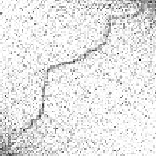
\includegraphics[width=120mm]{../img/walker.pdf}
\caption{A histogram of a generated matrix avoiding pattern~$P_1$.}
\label{walker}
\end{figure}

\begin{figure}[h!]
\centering
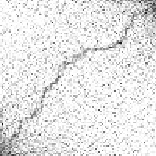
\includegraphics[width=120mm]{../img/walker2.pdf}
\caption{A histogram of a generated matrix avoiding pattern~$P_2$ using a different random seed than the previous picture.}
\label{walker2}
\end{figure}